\section{Introduction}

Linear regression is used to predict the value of an outcome variable (response) based on one or more input variables (predictor). The goal of linear regression model is to establish a linear relationship between predictors and responses. In this report, 

\section{Problem Formulation}

The aim of linear regression is to model the log returns of GM. $Y$ as a function of the log returns of Toyota $X_1$ and the log returns of Ford $X_2$. The function of their relationship can be defined as follows:
$$Y = \beta_0 + \beta_1 X_1 + \beta_2 X_2 + \epsilon$$
where $\beta_0$ is the intercept and $\beta_1$, $\beta_2$ are the regression coefficients of $X_1$, $X_2$ respectively. $\epsilon$ is the error term.

By definition of linear regression, the objective function for this problem is:

$$\min_{\beta} \norm{ Y - X \beta }^2_2 \iff \min_{\beta_0, \beta_1, \beta_2} \sum_{i=1}^{n} {(y_i - \beta_0 - \beta_1 x_{i1} - \beta_2 x_{i2})^2}$$


\section{Model Estimation}

A large number of procedures have been developed for parameter estimation inference in linear regression. Those methods are different in some aspects like computational simplicity, presence of a closed-form solution, robustness with respect to heavy-tailed distributions, etc. In this report, we apply the simplest and thus most common estimator to our linear regression model, ordinary least squares (OLS), which is the exact way how we estimate parameters in R. 

The OLS method minimizes the sum of squared residuals, and leads to a closed-form expression for the estimated value of the unknown parameter $\beta$:

$$\hat{\beta} = (\mathbf{X}^\top \mathbf{X})^{-1} \mathbf{X}^\top \mathbf{Y} = (\sum{\mathbf{x}_i\mathbf{x}_i^\top})^{-1} (\sum{\mathbf{x}_i} y_i) $$ 

In addition, the OLS estimaor is also identical to the maximum likelihood estimator (MLE) under the normality assumption for the error terms \cite{Abril07} (i.e. if the errors are i.i.d normal distribution $\mathcal{N}(0, \sigma^2)$.) 

% in the Bibliography section of your
% article will occur throughout the text of your article.
% You should use BibTeX to automatically produce this bibliography;
% you simply need to insert one of several citation commands with
% a key of the item cited in the proper location in
% the \texttt{.tex} file~\cite{Lamport:LaTeX}.
% The key is a short reference you invent to uniquely
% identify each work; in this sample document, the key is
% the first author's surname and a
% word from the title.  This identifying key is included
% with each item in the \texttt{.bib} file for your article.

% Immediately following this sentence is the point at which
% Table~\ref{tab:freq} is included in the input file; compare the
% placement of the table here with the table in the printed
% output of this document.

% \begin{table}
%   \caption{Frequency of Special Characters}
%   \label{tab:freq}
%   \begin{tabular}{ccl}
%     \toprule
%     Non-English or Math&Frequency&Comments\\
%     \midrule
%     \O & 1 in 1,000& For Swedish names\\
%     $\pi$ & 1 in 5& Common in math\\
%     \$ & 4 in 5 & Used in business\\
%     $\Psi^2_1$ & 1 in 40,000& Unexplained usage\\
%   \bottomrule
% \end{tabular}
% \end{table}

% \subsection{Figures}

\section{Experiments}

In experiments, we use the dataset provided on class that comes with R. Before begin building the linear regression model, we start to take a look at the raw dataset first to analyze and understand the variables intuitively. 



\begin{figure}
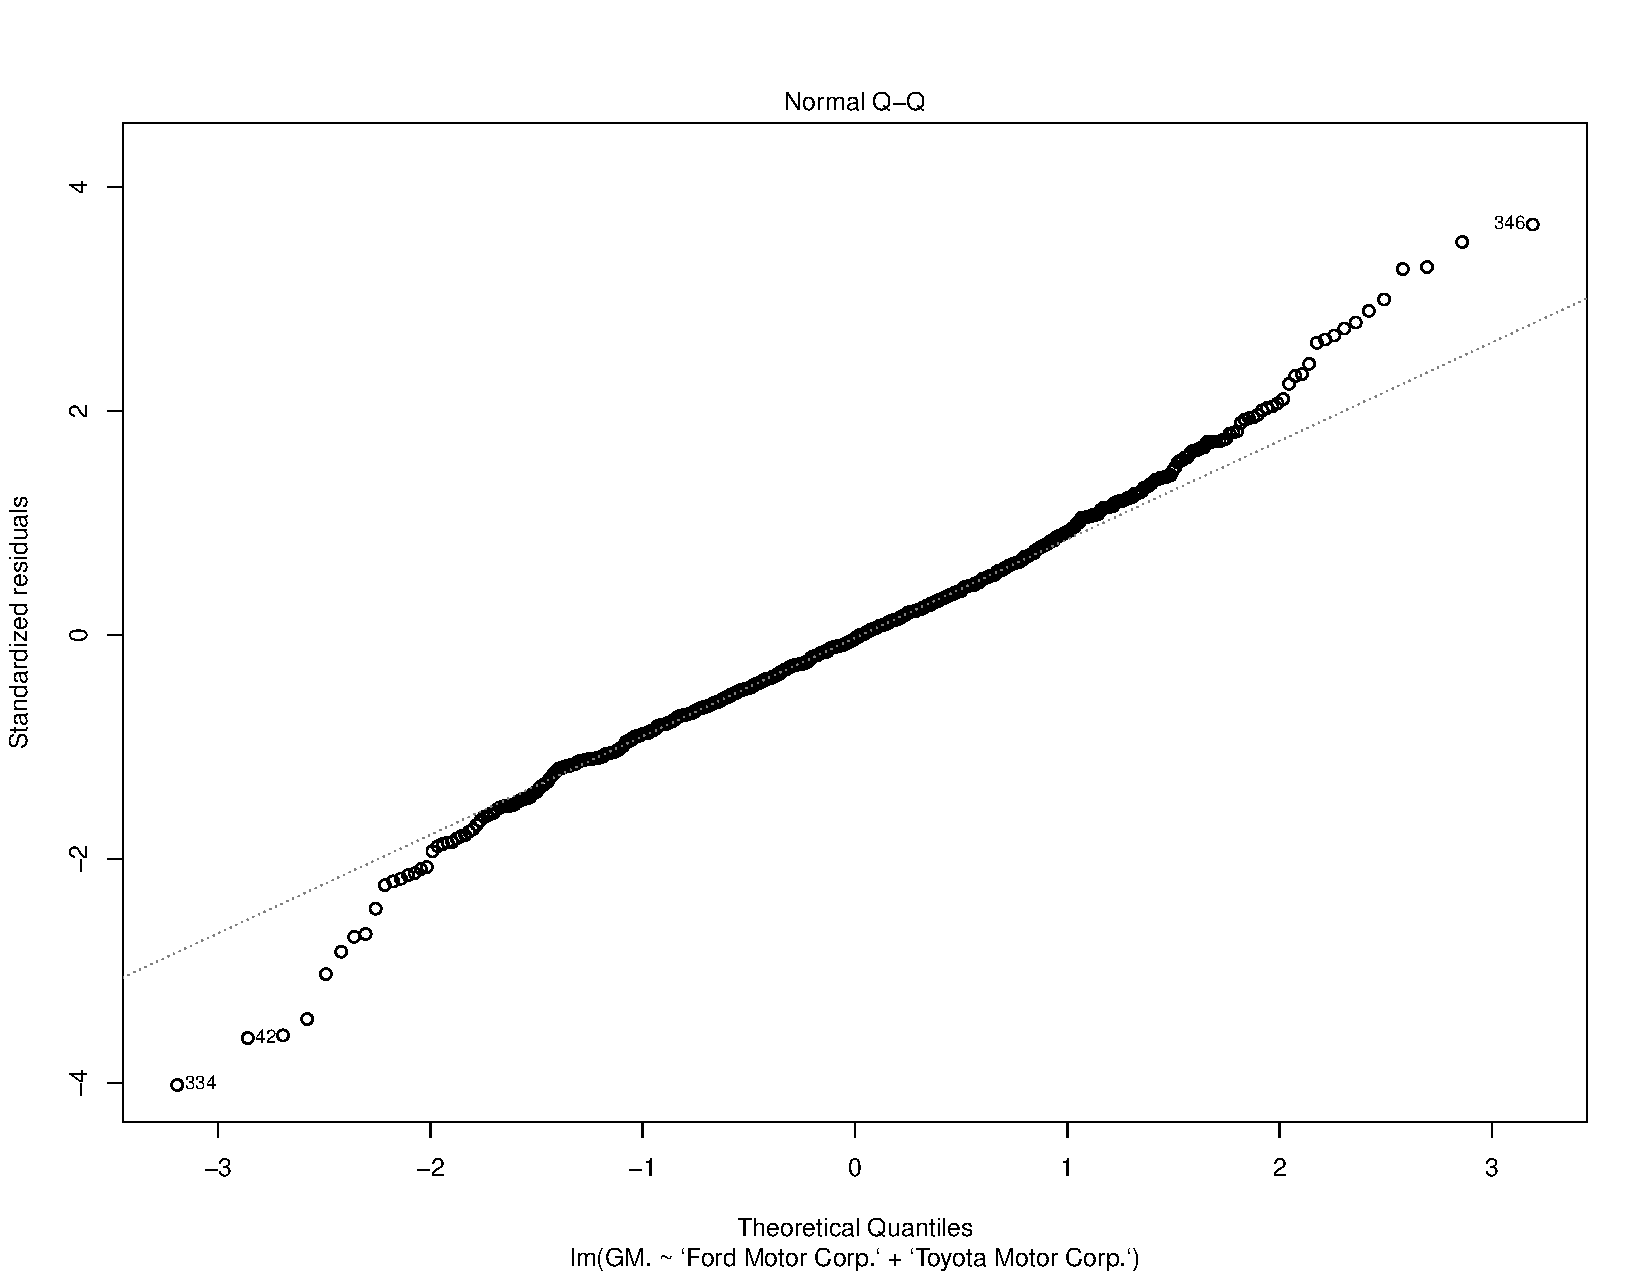
\includegraphics[height=3in, width=3in]{qqplot}
\caption{Normal Q-Q Plot}
\end{figure}

\begin{figure}
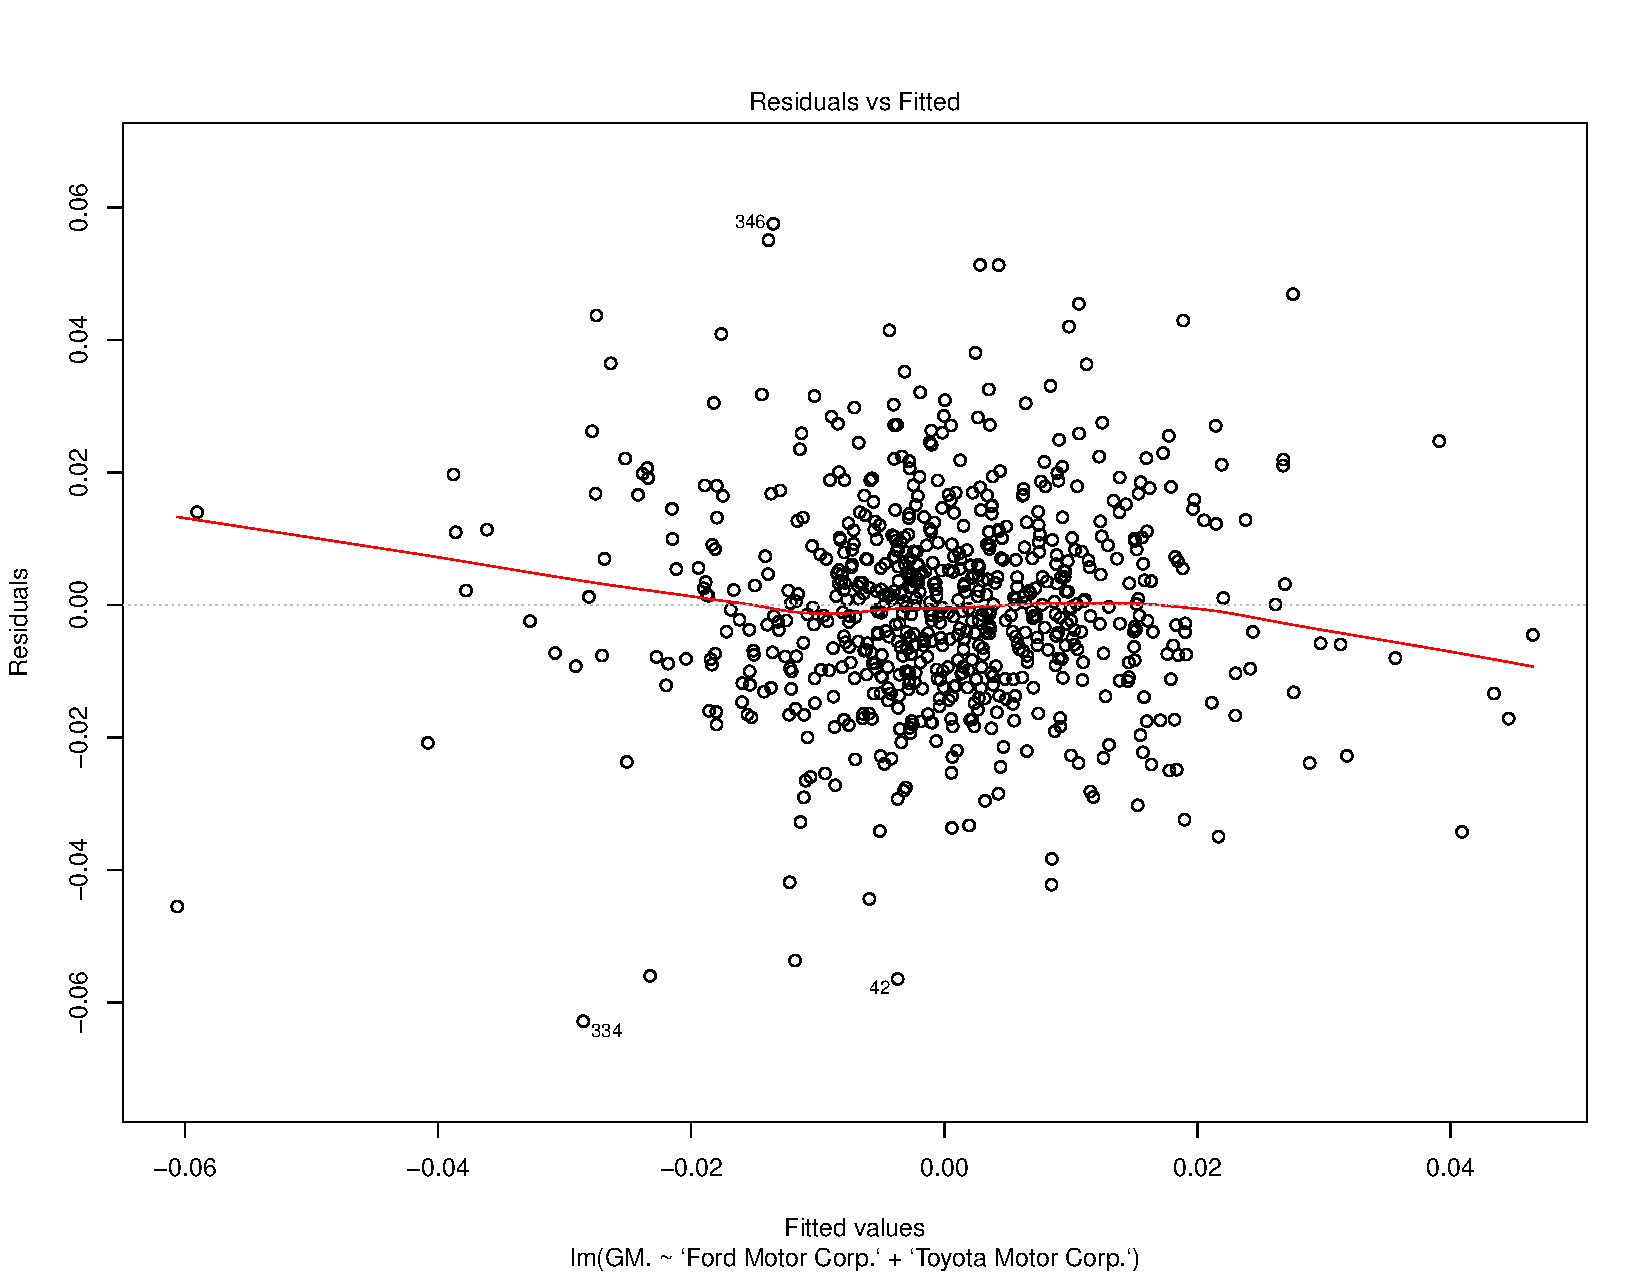
\includegraphics[height=3in, width=3in]{residuals-fitted}
\caption{Residuals-Fitted Plot}
\end{figure}

\begin{figure}
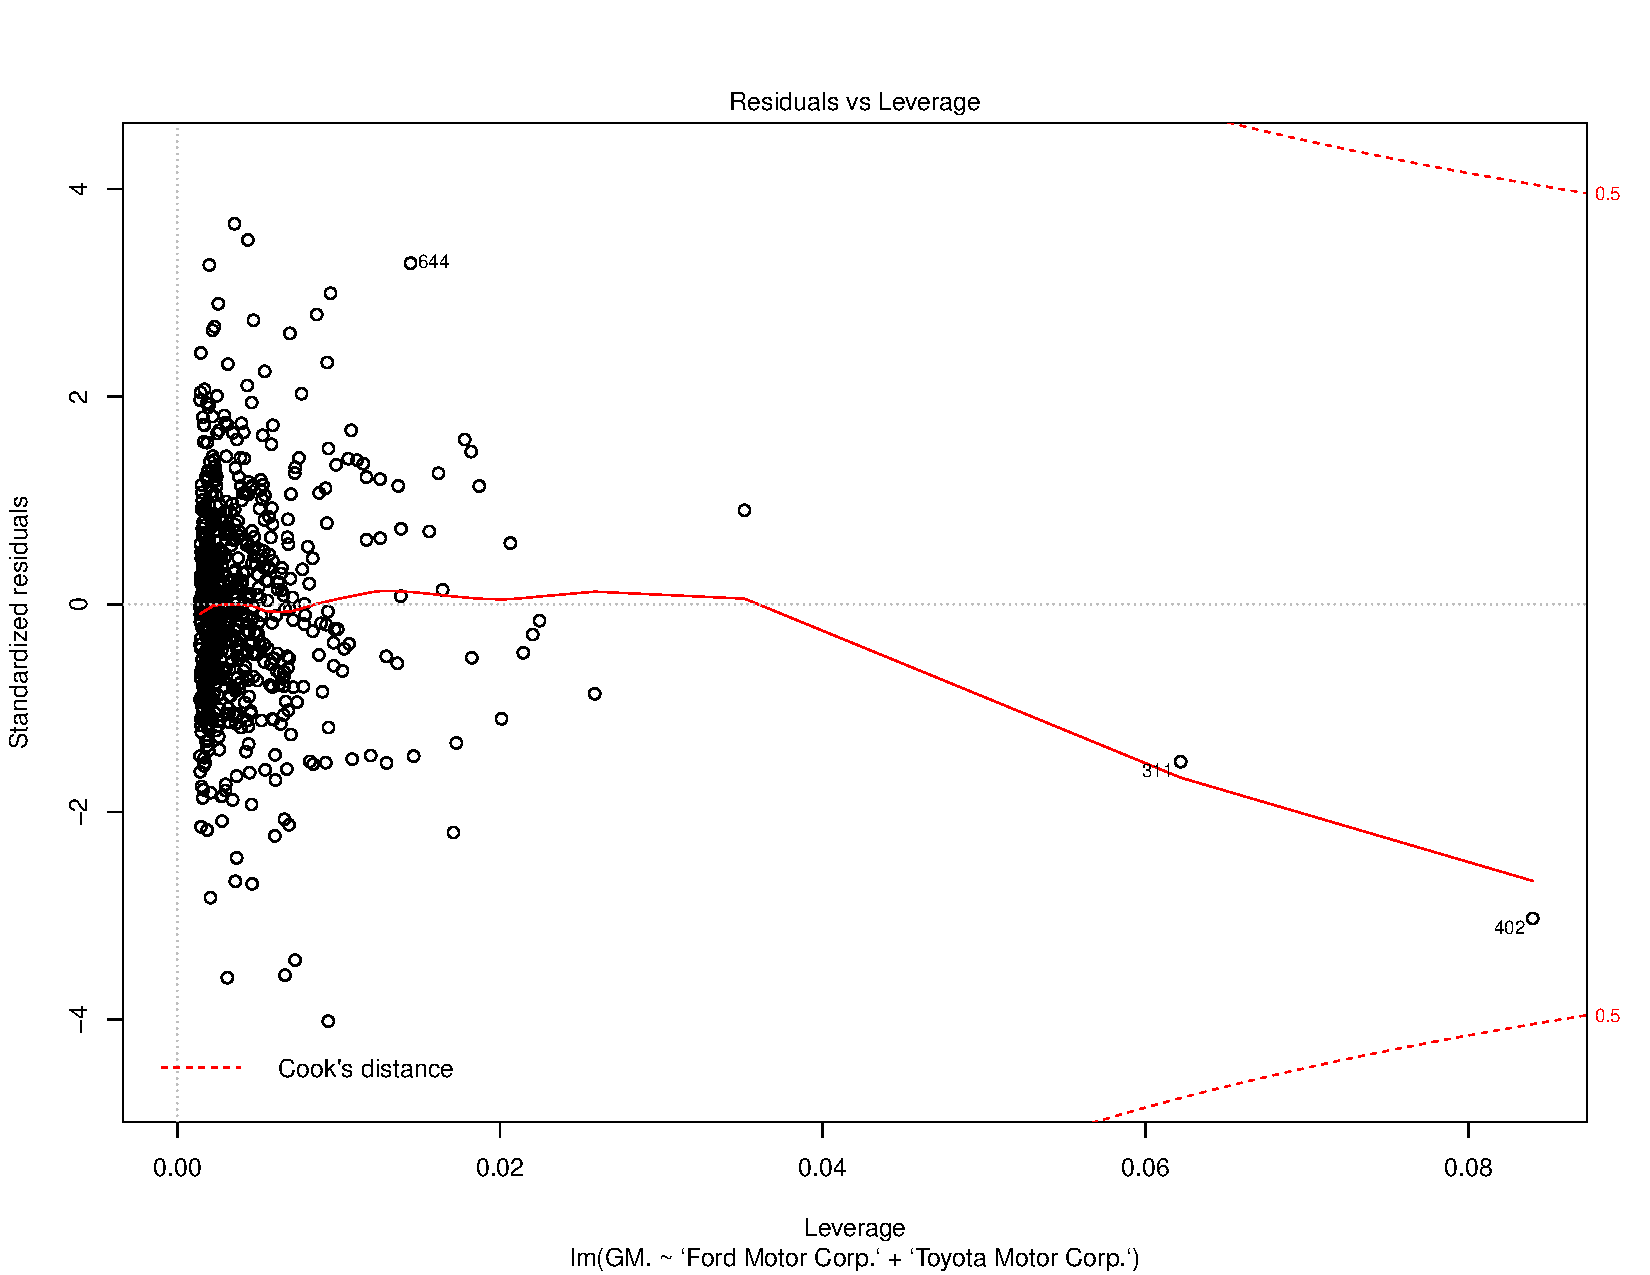
\includegraphics[height=3in, width=3in]{residuals-leverage}
\caption{Residuals-Leverage Plot}
\end{figure}

\begin{figure}
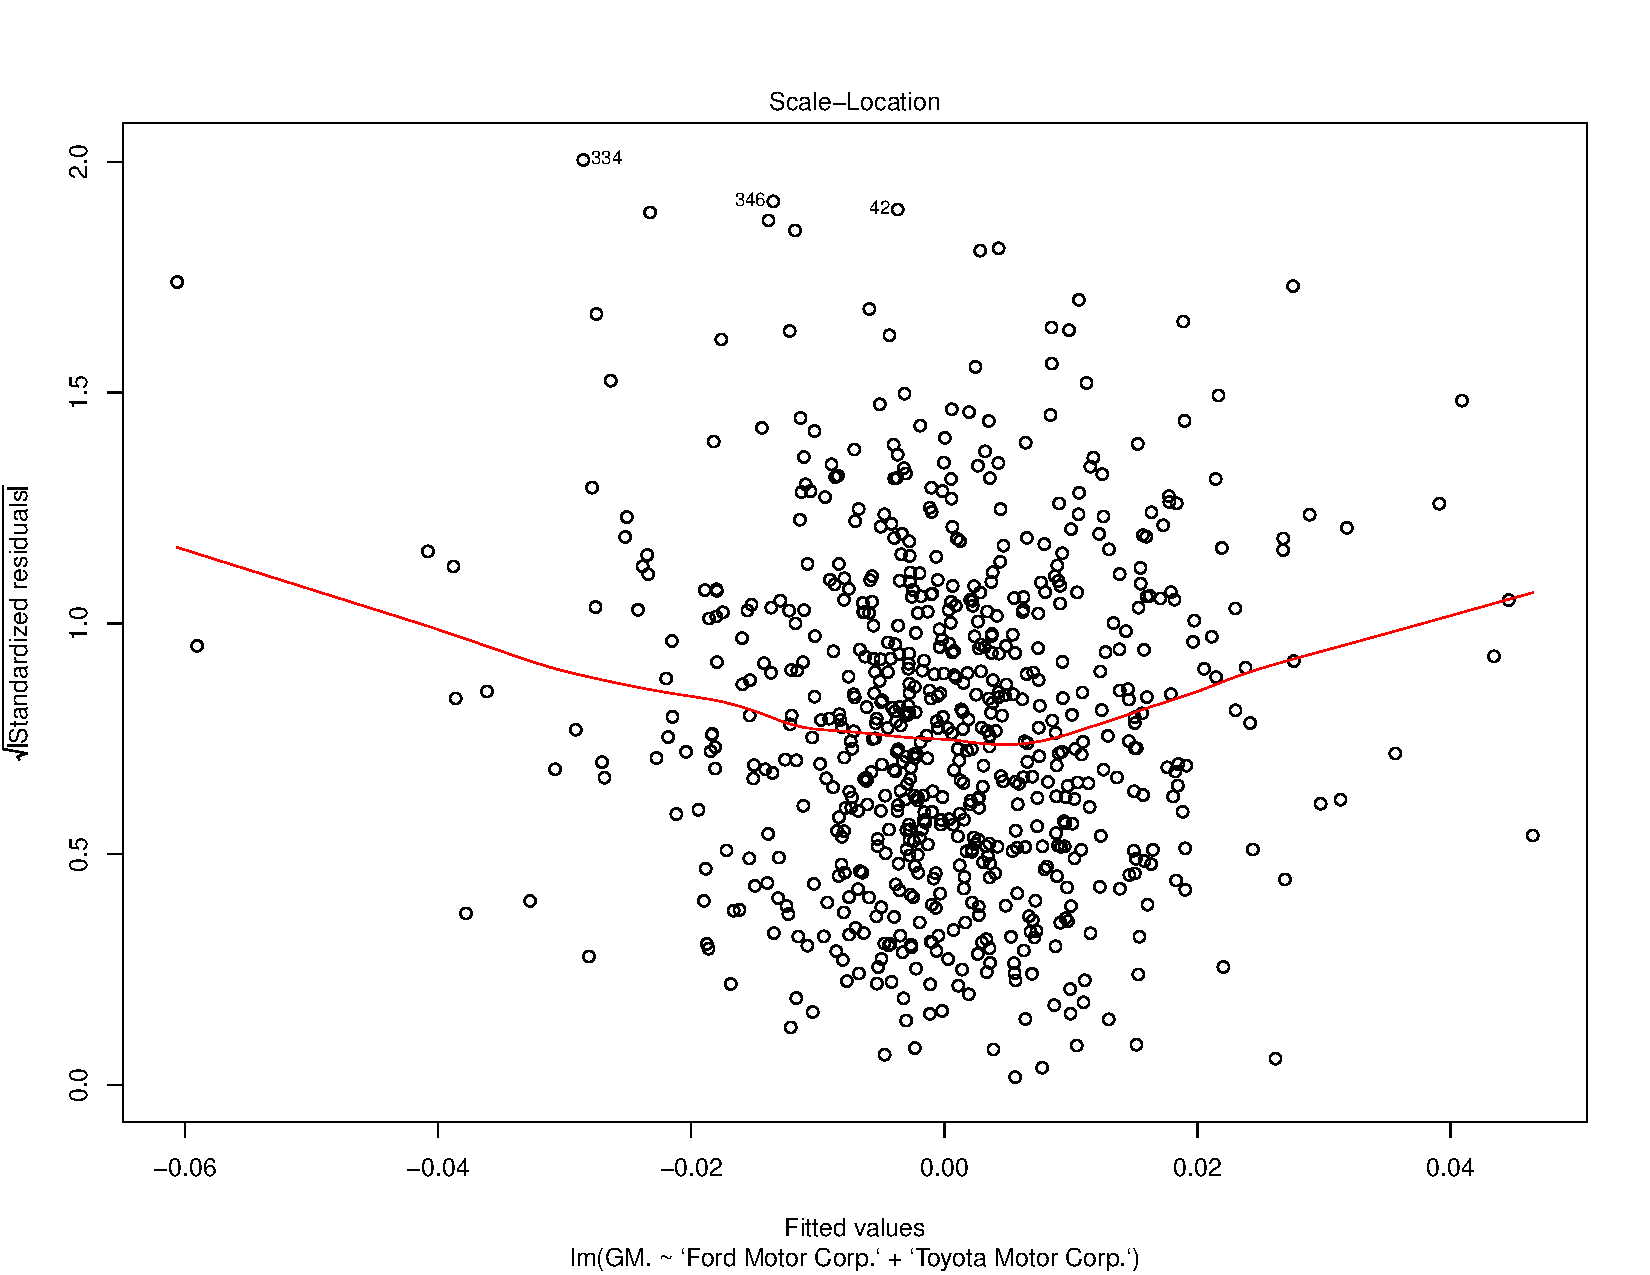
\includegraphics[height=3in, width=3in]{scale-location}
\caption{Scale-Location Plot}
\end{figure}

% \begin{figure}
% \includegraphics[height=1in, width=1in]{fly}
% \caption{A sample black and white graphic
% that has been resized with the \texttt{includegraphics} command.}
% \end{figure}

% \begin{figure*}
% \includegraphics{flies}
% \caption{A sample black and white graphic
% that needs to span two columns of text.}
% \end{figure*}

% \begin{figure}
% \includegraphics[height=1in, width=1in]{rosette}
% \caption{A sample black and white graphic that has
% been resized with the \texttt{includegraphics} command.}
% \end{figure}

% Here is a theorem:
% \begin{theorem}
%   Let $f$ be continuous on $[a,b]$.  If $G$ is
%   an antiderivative for $f$ on $[a,b]$, then
%   \begin{displaymath}
%     \int^b_af(t)\,dt = G(b) - G(a).
%   \end{displaymath}
% \end{theorem}

% Here is a definition:
% \begin{definition}
%   If $z$ is irrational, then by $e^z$ we mean the
%   unique number that has
%   logarithm $z$:
%   \begin{displaymath}
%     \log e^z = z.
%   \end{displaymath}
% \end{definition}

% \begin{proof}
%   Suppose on the contrary there exists a real number $L$ such that
%   \begin{displaymath}
%     \lim_{x\rightarrow\infty} \frac{f(x)}{g(x)} = L.
%   \end{displaymath}
%   Then
%   \begin{displaymath}
%     l=\lim_{x\rightarrow c} f(x)
%     = \lim_{x\rightarrow c}
%     \left[ g{x} \cdot \frac{f(x)}{g(x)} \right ]
%     = \lim_{x\rightarrow c} g(x) \cdot \lim_{x\rightarrow c}
%     \frac{f(x)}{g(x)} = 0\cdot L = 0,
%   \end{displaymath}
%   which contradicts our assumption that $l\neq 0$.
% \end{proof}

\section{Conclusions}
This paragraph will end the body of this sample document.
Remember that you might still have Acknowledgments or
Appendices; brief samples of these
follow.  There is still the Bibliography to deal with; and
we will make a disclaimer about that here: with the exception
of the reference to the \LaTeX\ book, the citations in
this paper are to articles which have nothing to
do with the present subject and are used as
examples only.
%\end{document}  % This is where a 'short' article might terminate
